\documentclass{article}
\usepackage{spconf,amsmath,epsfig,graphicx}
\usepackage{url}

\let\OLDthebibliography\thebibliography
\renewcommand\thebibliography[1]{
  \OLDthebibliography{#1}
  \setlength{\parskip}{0pt}
  \setlength{\itemsep}{0pt plus 0.3ex}
}

\pagestyle{empty}

\begin{document}\sloppy

\def\x{{\mathbf x}}
\def\L{{\cal L}}
\def\method{{Spectral-GS}}

\title{SPECTRAL-GS REPRODUCTION FOR ZOOM-ROBUST 3D GAUSSIAN SPLATTING}

\name{530182911 / yliu7029 \qquad 540433784 / sili0968 \qquad 550294609 / yche0218}
\address{COMP5405/4405 Digital Media Computing Project}

\maketitle

\begin{abstract}
3D Gaussian Splatting (3D-GS) enables fast high-quality novel-view synthesis, but it can produce needle-like artifacts when rendered at zoomed-in viewpoints. This project reproduces the main idea of Spectral-GS, which analyzes the covariance spectrum of 3D Gaussian primitives and uses spectral entropy to control Gaussian shape. We extend an existing 3D-GS codebase with covariance spectral entropy metrics, low-entropy shape-aware splitting, anisotropic scale reduction, a view-adaptive 2D filtering approximation, zoom-factor rendering, and metric reporting. Experiments on four real scenes show that the baseline remains stronger at the original scale, while the reproduced Spectral-GS branch improves robustness under zoom-in rendering. At 4x zoom, our implementation improves average PSNR by 1.59 dB, SSIM by 0.037, and LPIPS by 0.027 over the baseline 3D-GS. An additional ablation on two scenes shows that split-only training increases covariance entropy, while the full model best handles zoom artifacts.
\end{abstract}

\begin{keywords}
3D Gaussian Splatting, novel view synthesis, spectral entropy, zoom-in rendering, densification
\end{keywords}

\section{Introduction}
\label{sec:intro}

Novel-view synthesis is an important media computing task for computer graphics, virtual reality, augmented reality, digital twins, and 3D content creation. Given a set of calibrated images, the goal is to synthesize visually plausible images from new camera viewpoints. Neural radiance fields (NeRF) \cite{mildenhall2020nerf} demonstrated high-quality continuous scene representations, but their rendering and training costs are still inconvenient for interactive applications. 3D Gaussian Splatting (3D-GS) \cite{kerbl20233dgs} addresses this limitation by representing the scene as anisotropic 3D Gaussian primitives and rasterizing them efficiently, enabling real-time rendering with competitive visual quality.

However, high rendering speed does not remove all reconstruction artifacts. A known failure case of 3D-GS is the appearance of thin needle-like Gaussians, especially around high-frequency regions and zoomed-in views. These degenerated shapes may fit the training images but become unstable under a changed sampling rate. Spectral-GS \cite{huang2024spectralgs} observes that these problematic Gaussians are characterized by low spectral entropy and high condition number in their covariance matrices. It proposes two core changes: 3D shape-aware splitting based on covariance spectral entropy, and 2D view-consistent filtering for zoom-in rendering.

Our project is a reproduction-oriented implementation of Spectral-GS on top of an existing 3D-GS repository. The application target is zoom-robust real-time radiance-field rendering. The technical goal is not to build a new renderer from scratch, but to identify the missing paper components in the inherited codebase, implement the central Spectral-GS mechanisms, and evaluate whether the reproduced version improves zoomed-in novel-view quality.

\section{Related Work}
\label{sec:related}

NeRF \cite{mildenhall2020nerf} models a scene as a continuous radiance field and uses volume rendering to synthesize novel views. Follow-up work improved quality and anti-aliasing, including Mip-NeRF 360 \cite{barron2022mipnerf360}, but many NeRF-style methods require expensive network training and slow per-pixel rendering.

3D-GS \cite{kerbl20233dgs} replaces implicit neural fields with explicit anisotropic Gaussian primitives. Each Gaussian stores position, opacity, color represented by spherical harmonics, and a covariance matrix parameterized by scale and rotation. Adaptive densification clones or splits Gaussians according to view-space position gradients and primitive size. This design gives high rendering speed, but its densification rule does not directly penalize degenerated Gaussian shape.

Several methods study aliasing or filtering for Gaussian splatting. Mip-Splatting \cite{yu2024mipsplatting} introduces 3D smoothing and 2D Mip filtering to reduce aliasing, while Analytic-Splatting \cite{liang2024analyticsplatting} further analyzes the rendering and filtering process. Spectral-GS \cite{huang2024spectralgs} differs by explicitly analyzing the covariance spectrum and using spectral entropy to identify shape degeneration. This project focuses on reproducing the two Spectral-GS components that are most directly connected to the paper claim: covariance shape-aware splitting and view-consistent filtering.

\section{Methodology}
\label{sec:method}

Figure \ref{fig:methodology} summarizes the technical mechanism we reproduce from Spectral-GS. The 3D path is implemented as covariance spectral entropy based splitting with anisotropic scale shrinkage. The 2D path is implemented with the paper's scalar view-adaptive approximation, while the full matrix-form filter and full paper-scale benchmark remain limitations.

\begin{figure*}[t]
\centering
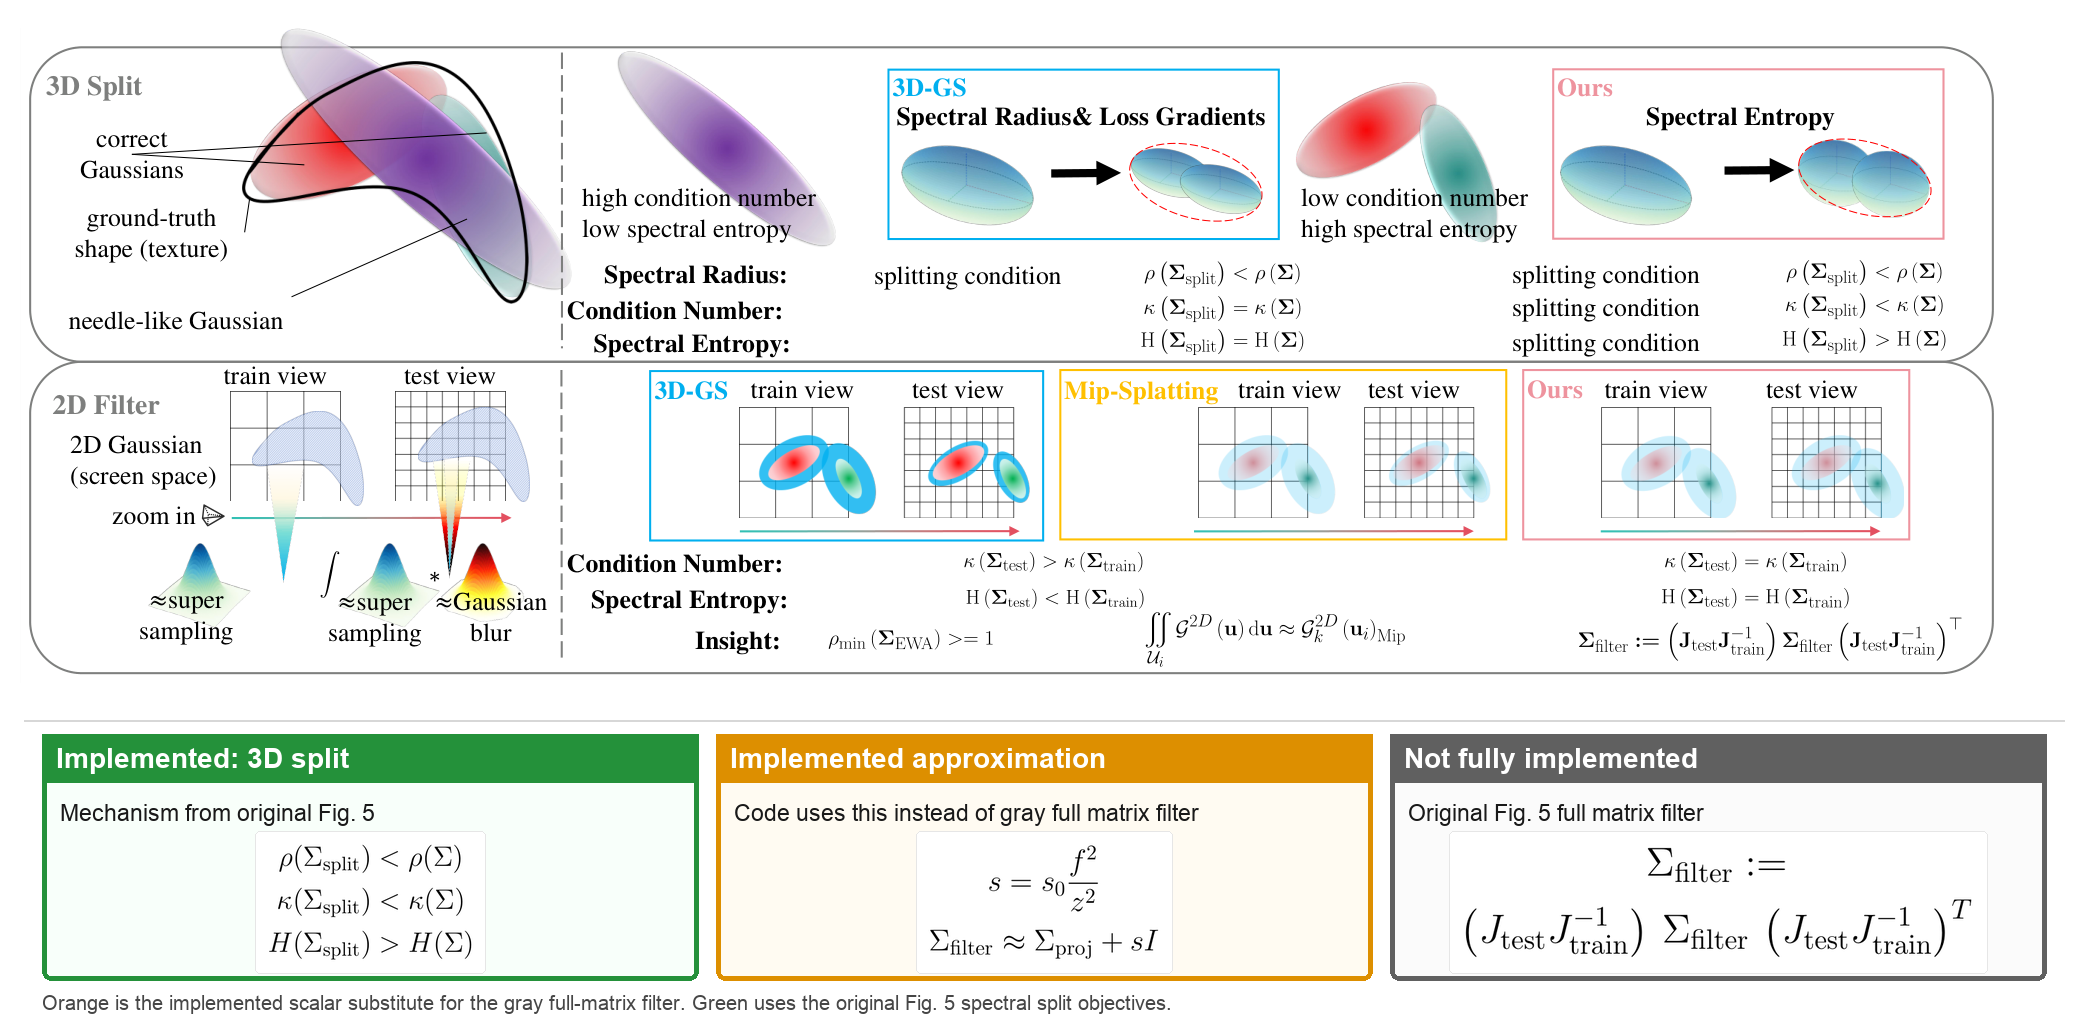
\includegraphics[width=0.98\textwidth]{figures/methodology_spectralgs_annotated.png}
\caption{Methodology overview adapted from Spectral-GS Figure 5 \cite{huang2024spectralgs}. The green box uses the original Figure 5 spectral split objectives. The orange box is the implemented scalar substitute for the gray full-matrix filter, which remains outside the current implementation. The methodology text writes the corresponding additive covariance form from the paper text.}
\label{fig:methodology}
\end{figure*}

\subsection{Baseline 3D Gaussian Splatting}

The baseline follows 3D-GS. A 3D Gaussian primitive is defined by mean $\mu$, opacity $o$, spherical harmonic color coefficients, and a covariance matrix
\begin{equation}
    \Sigma = R S S^T R^T,
\end{equation}
where $R$ is a rotation matrix and $S=\mathrm{diag}(s_1,s_2,s_3)$ stores the learned scale parameters. The primitive is projected to screen space by a local affine Jacobian $J$ and camera transform $W$:
\begin{equation}
    \Sigma_{proj}=J W \Sigma W^T J^T.
\end{equation}
Training optimizes an image reconstruction loss combining L1 and D-SSIM, while adaptive densification changes the number of primitives. In the original 3D-GS rule, Gaussians with high view-space positional gradients are cloned or split depending on their scale.

\subsection{Covariance spectral metrics}

Spectral-GS treats the covariance eigenvalues as a compact description of Gaussian shape. Since $\Sigma=R S S^T R^T$, the covariance eigenvalues are $s_1^2$, $s_2^2$, and $s_3^2$. We compute normalized eigenvalue probabilities
\begin{equation}
    p_i=\frac{s_i^2}{s_1^2+s_2^2+s_3^2},
\end{equation}
and define spectral entropy
\begin{equation}
    H(\Sigma)=-\sum_{i=1}^{3}p_i\log p_i.
\end{equation}
Low entropy indicates that most covariance energy lies on one axis, which corresponds to an elongated Gaussian. We also compute the condition number
\begin{equation}
    \kappa(\Sigma)=\frac{\max_i s_i^2}{\min_i s_i^2}
\end{equation}
and spectral radius $\rho(\Sigma)=\max_i s_i^2$ for logging and analysis.

\subsection{Shape-aware splitting}

The inherited project already contained a DCT-based spectral loss and a spectral densification heuristic, but this was not the main mechanism in Spectral-GS. We replaced the main paper reproduction path with covariance-entropy splitting. During densification, a Gaussian is eligible for splitting either because it satisfies the original 3D-GS gradient rule or because its covariance entropy is below a threshold:
\begin{equation}
    H(\Sigma) < \tau_{spectral}.
\end{equation}
We use the paper default $\tau_{spectral}=0.5$. This makes splitting independent of the image loss gradient for low-entropy Gaussians, which is important because needle-like primitives can fit the training view while having small positional gradients.

The implementation preserves the original 3D-GS clone/split size gate and adds the spectral split mask to the large-Gaussian split path. Let $p$ be \texttt{percent\_dense}, $E$ be the scene extent, and $s_{\max}=\max(s)$. The densification masks are
\begin{equation}
\begin{aligned}
M_{\mathrm{clone}} &=
\mathbf{1}\{\|\nabla_{\mu_{\mathrm{proj}}}L\|\ge\tau_{\mathrm{loss}}\}
\land \mathbf{1}\{s_{\max}\le pE\},\\
M_{\mathrm{grad\_split}} &=
\mathbf{1}\{\|\nabla_{\mu_{\mathrm{proj}}}L\|\ge\tau_{\mathrm{loss}}\}
\land \mathbf{1}\{s_{\max}>pE\},\\
M_{\mathrm{spec\_split}} &=
\mathbf{1}\{H(\Sigma)<\tau_{\mathrm{spectral}}\}
\land \mathbf{1}\{s_{\max}>pE\},\\
M_{\mathrm{split}} &= M_{\mathrm{grad\_split}}\lor M_{\mathrm{spec\_split}}.
\end{aligned}
\end{equation}
Thus, small high-gradient Gaussians are cloned, while large high-gradient or low-entropy Gaussians are split. Gradient-only split keeps the 3D-GS scale rule $s'=s/(0.8N)$. Spectral-selected split instead uses the dominant-axis shrink
\begin{equation}
    i^*=\arg\max_i s_i^2,\quad
    s_{i^*}'=\frac{s_{i^*}}{k_0+\delta},\quad
    s_j'=\frac{s_j}{k_0}\;(j\ne i^*).
\end{equation}
After split children are inserted, the selected parent Gaussians are removed and the standard opacity/radius pruning step is still applied.

For Gaussians selected by the spectral condition, the split is anisotropic. Instead of uniformly shrinking every axis, we shrink the dominant covariance axis more strongly. With $K=2$, $k_0=1.0$, and $\delta=0.6$, the dominant scale is divided by $k_0+\delta=1.6$ and the other axes are divided by $k_0$. This follows the paper's practical parameters and is intended to reduce condition number while preserving local high-frequency support.

\subsection{View-consistent filtering}

The original CUDA rasterizer uses a fixed EWA-style 2D filter variance,
\begin{equation}
    \Sigma_{filter}=\Sigma_{proj}+sI,\quad s=0.3.
\end{equation}
Spectral-GS argues that this constant filter becomes view-inconsistent when focal length or depth changes, causing the 2D Gaussian condition number to change during zoom-in rendering. The two equalities shown above the filter formula in Figure \ref{fig:methodology},
\begin{equation}
    \kappa(\Sigma_{test})=\kappa(\Sigma_{train}), \quad H(\Sigma_{test})=H(\Sigma_{train}),
\end{equation}
are target properties rather than separate implementation steps: the filtered 2D covariance should keep the same condition number and spectral entropy between training and zoomed test views. The full paper derives a matrix-form view-consistent filter to enforce this behavior,
\begin{equation}
    \Sigma_{filter}=\Sigma_{proj}+(J_{test}J_{train}^{-1})sI(J_{test}J_{train}^{-1})^T.
\end{equation}
The paper also states that this can be approximated with a scalar function of focal length and depth. Our implementation uses this practical approximation:
\begin{equation}
    s=s_0\frac{f^2}{z^2},
\end{equation}
where $f$ is the average focal length and $z$ is camera-space depth. The CUDA rasterizer exposes this behavior through \texttt{--use\_view\_consistent\_filter} and \texttt{--spectral\_filter\_s0}. We choose $s_0$ by matching the scalar filter to the baseline variance near the training-view operating point:
\begin{equation}
    s_0 \approx 0.3\left(\frac{z_{\mathrm{train}}}{f_{\mathrm{train}}}\right)^2.
\end{equation}
For the downsampled scenes used in our experiments, this places $s_0$ around $10^{-5}$ to $10^{-4}$, so we use $s_0=0.0001$. The paper reports $s_0=0.1$, but that value is too large for the current rasterizer and resolution setting and causes excessive blur. This calibration is a practical scalar substitute, not a full implementation of the matrix filter above.

\subsection{Zoom-in evaluation}

To test robustness to changed sampling rate, we added a \texttt{--zoom\_factor} option to the rendering script. For a zoom factor $q$, the renderer shrinks the camera field of view by increasing the effective focal length, the GT image is center-cropped to the corresponding $1/q$ region, and the crop is resized back to the original resolution before PSNR, SSIM, and LPIPS are computed. We evaluate at 1x, 2x, and 4x zoom.

\section{Implementation}
\label{sec:implementation}

The implementation was developed on a new branch named \texttt{spectral-gs-full-paper}. The main changes are summarized below.

\begin{itemize}
    \item \texttt{utils/spectral\_utils.py}: covariance spectral entropy, condition number, and spectral radius from activated 3D Gaussian scales.
    \item \texttt{scene/gaussian\_model.py}: low-entropy splitting mask, gradient-independent spectral split trigger, and anisotropic dominant-axis scale reduction.
    \item Rasterization submodule: Python and CUDA arguments for view-consistent filtering, plus forward and backward use of $s_0 f^2/z^2$.
    \item \texttt{render.py}: zoom-factor rendering and matched ground-truth crop generation.
    \item \texttt{metrics.py}: per-method metric export and Gaussian entropy/condition statistics when point-cloud checkpoints are available.
    \item \texttt{SPECTRAL\_GS\_REPRODUCTION.md}: reproduction notes and runnable training commands.
\end{itemize}

The baseline path is preserved: if the new Spectral-GS flags are disabled, training and rendering follow the inherited 3D-GS behavior. A typical baseline command is:
\begin{quote}
\small
\texttt{python train.py -s data/truck -m output/truck\_baseline\_r2 -r 2 --eval --iterations 15000}
\end{quote}
The reproduced Spectral-GS command is:
\begin{quote}
\small
\texttt{python train.py -s data/truck -m output/truck\_full\_r2 -r 2 --eval --iterations 15000 --use\_spectral\_shape\_split --use\_view\_consistent\_filter --spectral\_filter\_s0 0.0001}
\end{quote}

\section{Experiments}
\label{sec:experiments}

\subsection{Experimental setup}

We evaluate on four real scenes: \texttt{truck}, \texttt{train}, \texttt{drjohnson}, and \texttt{playroom}. The \texttt{truck} and \texttt{train} scenes are standard real 3D-GS benchmark scenes, while \texttt{drjohnson} and \texttt{playroom} are Deep Blending style indoor scenes. All experiments use image downsampling \texttt{-r 2} and 15000 training iterations. The four-scene main comparison uses the baseline and full Spectral-GS setting, while a two-scene ablation on \texttt{truck} and \texttt{playroom} also reports split-only results. The compared settings are:

\begin{itemize}
    \item \textbf{Baseline}: inherited 3D-GS training and the standard rasterizer.
    \item \textbf{Split}: 3D covariance entropy shape-aware splitting without the view-consistent filter.
    \item \textbf{Full}: split plus view-consistent filtering with \texttt{--spectral\_filter\_s0 0.0001}.
\end{itemize}

We report PSNR, SSIM, LPIPS \cite{zhang2018lpips}, and covariance entropy. PSNR measures pixel-level reconstruction accuracy through mean squared error, so higher is better. SSIM measures structural similarity in luminance, contrast, and local structure, so higher is better. LPIPS measures learned perceptual distance between the render and the reference image, so lower is better. EntropyMean is the mean 3D covariance spectral entropy of the saved Gaussians; higher values generally indicate less needle-like shape degeneration, although it is not an image-quality metric by itself. GT denotes the ground-truth held-out image or matched zoom crop used as the reference for quantitative metrics and qualitative comparison. The metric scripts evaluate test renders at 1x, 2x, and 4x zoom.

\begin{table}[t]
\centering
\caption{Average comparison over four scenes. Best metric values are in bold. Spectral-GS is weaker at 1x but improves zoom-in robustness.}
\label{tab:avg}
\footnotesize
\begin{tabular}{llccc}
\hline
Metric & Zoom & Baseline & Spectral & Diff. \\
\hline
PSNR $\uparrow$ & 1x & \textbf{26.95} & 26.37 & -0.58 \\
PSNR $\uparrow$ & 2x & 26.10 & \textbf{27.01} & +0.91 \\
PSNR $\uparrow$ & 4x & 26.47 & \textbf{28.06} & +1.59 \\
SSIM $\uparrow$ & 1x & \textbf{0.903} & 0.875 & -0.028 \\
SSIM $\uparrow$ & 2x & 0.848 & \textbf{0.866} & +0.017 \\
SSIM $\uparrow$ & 4x & 0.859 & \textbf{0.896} & +0.037 \\
LPIPS $\downarrow$ & 1x & \textbf{0.134} & 0.174 & +0.040 \\
LPIPS $\downarrow$ & 2x & 0.181 & \textbf{0.176} & -0.004 \\
LPIPS $\downarrow$ & 4x & 0.214 & \textbf{0.187} & -0.027 \\
\hline
\end{tabular}
\end{table}

\begin{table}[t]
\centering
\caption{Per-scene PSNR at 4x zoom. Best values are in bold. Spectral-GS improves every tested scene under strong zoom-in rendering.}
\label{tab:zoom4}
\begin{tabular}{l|ccc}
\hline
Scene & Baseline & Spectral & Diff. \\
\hline
truck & 23.15 & \textbf{25.98} & +2.83 \\
train & 21.05 & \textbf{22.55} & +1.50 \\
drjohnson & 30.18 & \textbf{30.85} & +0.67 \\
playroom & 31.51 & \textbf{32.87} & +1.36 \\
\hline
Average & 26.47 & \textbf{28.06} & +1.59 \\
\hline
\end{tabular}
\end{table}

\begin{table}[t]
\centering
\caption{Ablation averaged over \texttt{truck} and \texttt{playroom}. Best metric values within each zoom group are in bold. Full combines split and view-consistent filtering.}
\label{tab:ablation}
\footnotesize
\begin{tabular}{llccc}
\hline
Zoom & Method & PSNR $\uparrow$ & SSIM $\uparrow$ & LPIPS $\downarrow$ \\
\hline
1x & Baseline & 28.25 & 0.923 & 0.118 \\
1x & Split & \textbf{28.36} & \textbf{0.927} & \textbf{0.109} \\
1x & Full & 27.87 & 0.915 & 0.130 \\
2x & Baseline & 27.29 & 0.860 & 0.168 \\
2x & Split & 27.31 & 0.861 & 0.165 \\
2x & Full & \textbf{28.61} & \textbf{0.889} & \textbf{0.142} \\
4x & Baseline & 27.33 & 0.867 & 0.208 \\
4x & Split & 27.39 & 0.868 & 0.207 \\
4x & Full & \textbf{29.42} & \textbf{0.911} & \textbf{0.153} \\
\hline
\end{tabular}
\end{table}

\begin{table}[t]
\centering
\caption{Mean covariance spectral entropy from the ablation scenes. Highest entropy values are in bold. Higher values indicate less degenerated Gaussian shapes.}
\label{tab:entropy}
\footnotesize
\begin{tabular}{lccc}
\hline
Scene & Baseline & Split & Full \\
\hline
truck & 0.3151 & 0.4732 & \textbf{0.5331} \\
playroom & 0.3141 & \textbf{0.3850} & 0.3219 \\
Average & 0.3146 & \textbf{0.4291} & 0.4275 \\
\hline
\end{tabular}
\end{table}

\begin{figure*}[t]
\centering
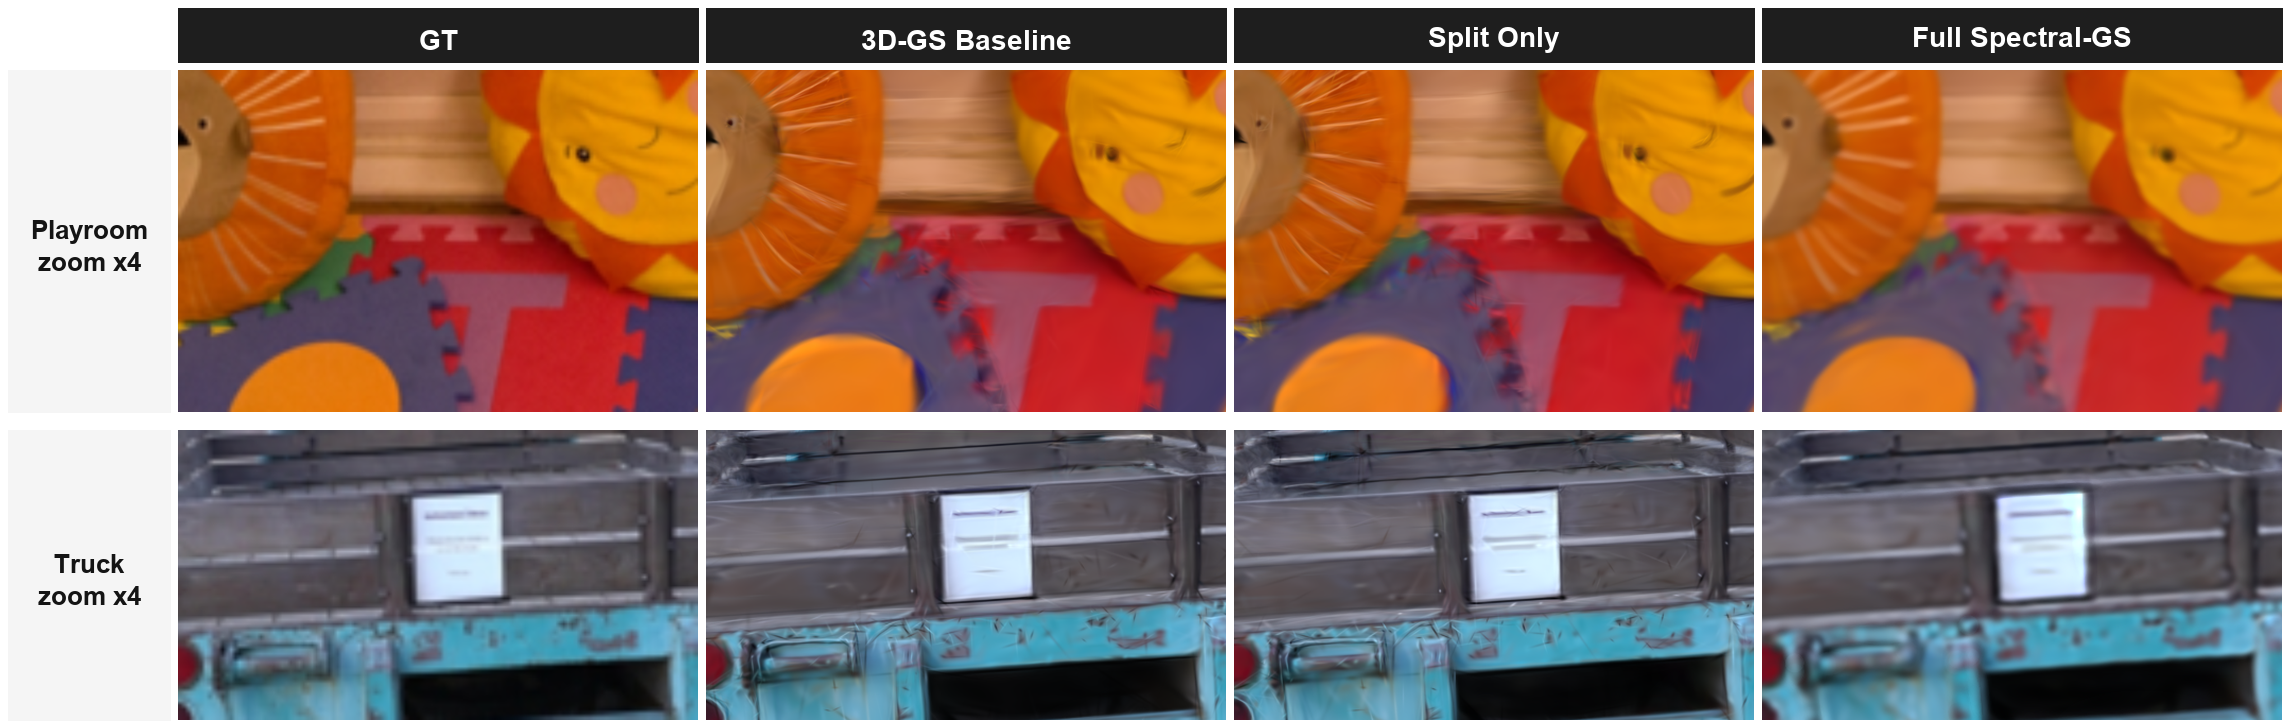
\includegraphics[width=0.98\textwidth]{figures/qualitative_zoom4_ablation.png}
\caption{Qualitative zoom 4x comparison on \texttt{playroom} and \texttt{truck}. GT is the matched ground-truth crop from the held-out image. Split-only training mainly regularizes Gaussian shape, while the full Spectral-GS setting combines shape-aware splitting and view-consistent filtering. The full setting reduces the most visible needle-like and streak artifacts under strong zoom-in rendering.}
\label{fig:qualitative}
\end{figure*}

\subsection{Results}

Table \ref{tab:avg} shows a clear tradeoff. At the original 1x view, the baseline 3D-GS is slightly better on average: PSNR is higher by 0.58 dB, SSIM is higher by 0.028, and LPIPS is lower by 0.040. This means our reproduced Spectral-GS settings do not simply improve all rendered images. The spectral constraints and adaptive filter change the training and rasterization behavior, and may reduce direct overfitting to the original test resolution.

At zoomed-in views, the result changes. At 2x zoom, Spectral-GS improves average PSNR by 0.91 dB and SSIM by 0.017, while LPIPS is slightly better. At 4x zoom, the advantage becomes stronger: PSNR improves by 1.59 dB, SSIM improves by 0.037, and LPIPS decreases by 0.027. Table \ref{tab:zoom4} confirms that every scene benefits at 4x zoom, with the largest PSNR gains on \texttt{truck} and \texttt{train}. These two outdoor scenes contain more high-frequency texture and edges, where needle-like Gaussian artifacts are easier to expose under zoom. The indoor scenes improve less, but still benefit at 4x. This matches the main claim of Spectral-GS: the method is designed to reduce zoom-induced artifacts rather than only maximize original-resolution metrics.

The ablation in Table \ref{tab:ablation} separates the two effects on \texttt{truck} and \texttt{playroom}. Split-only training slightly improves the 1x and 4x averages and increases mean spectral entropy, but the full setting is clearly stronger at zoomed-in views. At 4x zoom, Full reaches 29.42 PSNR, 0.911 SSIM, and 0.153 LPIPS, compared with 27.33 PSNR, 0.867 SSIM, and 0.208 LPIPS for the baseline. This suggests that shape-aware splitting helps regularize the 3D Gaussians, while the view-consistent filter is important for reducing artifacts caused by zoomed rendering.

Table \ref{tab:entropy} supports the intended shape effect. On \texttt{truck}, entropy rises from 0.3151 for the baseline to 0.4732 for Split and 0.5331 for Full. On \texttt{playroom}, Split also increases entropy, while Full gives the best zoomed image metrics without producing the largest entropy. This is consistent with the method design: the 3D split directly affects covariance shape, while the 2D filter mainly improves view consistency during rasterization. Figure \ref{fig:qualitative} gives the corresponding visual evidence. The baseline contains visible streak and needle-like artifacts in zoomed crops, Split reduces some shape degeneration, and Full produces the cleanest zoom-in results among the tested variants.

\section{Discussion and Limitations}
\label{sec:discussion}

This project implements the two central components of Spectral-GS, but it should be described as a faithful core reproduction rather than a complete paper-level reproduction. There are several limitations.

First, the 2D filter uses the paper's scalar approximation $s_0 f^2/z^2$, not the full matrix form involving $J_{test}J_{train}^{-1}$. The scalar version is easier to integrate into the existing CUDA rasterizer and is explicitly mentioned by the paper, but it cannot model direction-dependent anisotropic filtering as accurately as the full matrix expression.

Second, the experiment scale is smaller than the original paper. The paper evaluates 12 scenes and compares with 3D-GS, Mip-Splatting, Analytic-Splatting, and Analytic-Splatting with a 3D filter. Our final experiment uses four scenes for the main baseline-vs-full comparison and two scenes for the split ablation. This is sufficient to show the project behavior, but not enough to claim the same benchmark coverage as the paper.

Third, the runs use 15000 iterations rather than a full 30000-iteration setting. This is a practical compromise for course-project runtime. We also do not include a filter-only ablation or a runtime table, so the exact isolated contribution and cost of the 2D filter remain less completely characterized.

Finally, the inherited repository still contains the older DCT-based spectral loss path. It is useful as an inspired baseline, but it is not the mechanism proposed by Spectral-GS. In this report, the reported Spectral-GS setting refers to the new covariance entropy split and view-consistent filter flags.

\section{Reflection on AI Usage}
\label{sec:reflection}

AI tools were used as engineering assistants during the final stage. They helped inspect the existing codebase, compare it against the Spectral-GS paper, identify which implemented parts were not paper-faithful, draft the reproduction plan, modify source files, and structure this report according to the project rubric. The useful learning outcome was that the team had to translate paper equations into concrete implementation points: where Gaussian scales are stored, where densification decisions happen, where the CUDA rasterizer injects filter variance, and how zoom evaluation should pair renderings with ground truth.

The AI output was not treated as automatically correct. The team checked the implementation against the paper PDF, retained the original 3D-GS baseline path, ran the experiments separately, and used the measured metrics in the report. The main risk of AI assistance was overclaiming completeness. To avoid that, this report explicitly separates implemented core components from remaining paper-level gaps such as the full matrix filter and broader benchmark suite. A separate AI usage record PDF should be submitted with the project documents as required by the assignment.

\section{Team Contribution}
\label{sec:contribution}

The three listed group members contributed as an equal project team across literature review, implementation, experiment execution, report writing, and final presentation preparation. The final submission uses student IDs and unikeys instead of full names, following the assignment instruction.

\section{Conclusion}
\label{sec:conclusion}

We reproduced the core Spectral-GS idea in a 3D-GS codebase by adding covariance spectral entropy analysis, low-entropy shape-aware splitting, anisotropic split shrinkage, scalar view-consistent filtering, and zoom-factor evaluation. The final results show that the baseline is slightly better at 1x rendering, but the Spectral-GS branch is consistently stronger at 2x and 4x zoom. This supports the paper's central motivation: spectral shape awareness is most valuable when the sampling rate changes and needle-like artifacts become visible.

\bibliographystyle{IEEEbib}
\bibliography{final_report}

\end{document}
